\begin{figure}
	\centering
	\begin{subfigure}[b]{0.4\textwidth}
		
\includegraphics[width=\textwidth]{figures/circle.png}
		\caption{}
		\label{fig:circle}
	\end{subfigure}
	~~~
	\begin{subfigure}[b]{0.4\textwidth}
		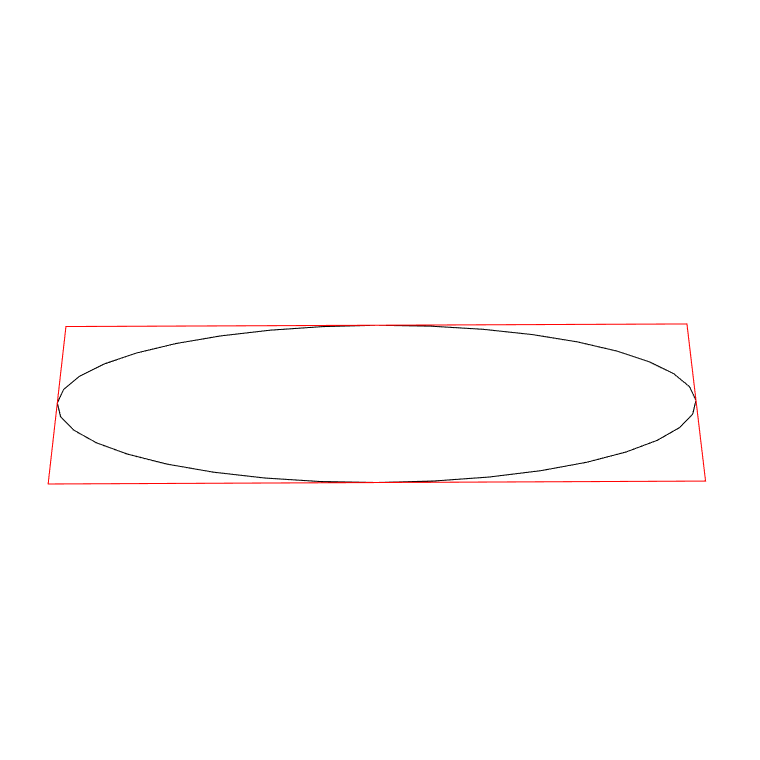
\includegraphics[width=\textwidth]{figures/circle_perspective.png}
		\caption{}
		\label{fig:circle_perspective}
	\end{subfigure}
		\caption{(a) A circle enclosed by a square. (b) The same circle and square, distorted by a projective transformation.}\label{fig:perspective}
\end{figure}